\chapter{Results}

\phantomsection
\section*{Toxicity dataset}
\addcontentsline{toc}{section}{Toxicity dataset}

The dataset showed a greater proportion of inactive labels as illustrated in Figure \ref{fig:bars_endpoints}. For the whole dataset, the average ratio of active/inactive labels was 8.6\% and average missing labels was 16.6\%. After filtering for the available mass spectra, these values changed to 12.1\% and 13.9\%, respectively. The frequency of labels for each endpoint is shown in Table \ref{table:labels_tox} and Table \ref{table:labels_tox_MassBank}.


The association of binary classification between endpoints was investigated. The phi coefficient ranged from 0.013 (NR.AR, NR.PPAR.gamma) to 0.756 (NR.AR, NR.AR.LBD). An additional high phi coefficient was 0.7405 (NR.ER, NR.ER.LBD). The phi coefficients for all the pairs are illustrated in Figure \ref{fig:phi_coefficient}.

\begin{figure}[H]
	\centering
  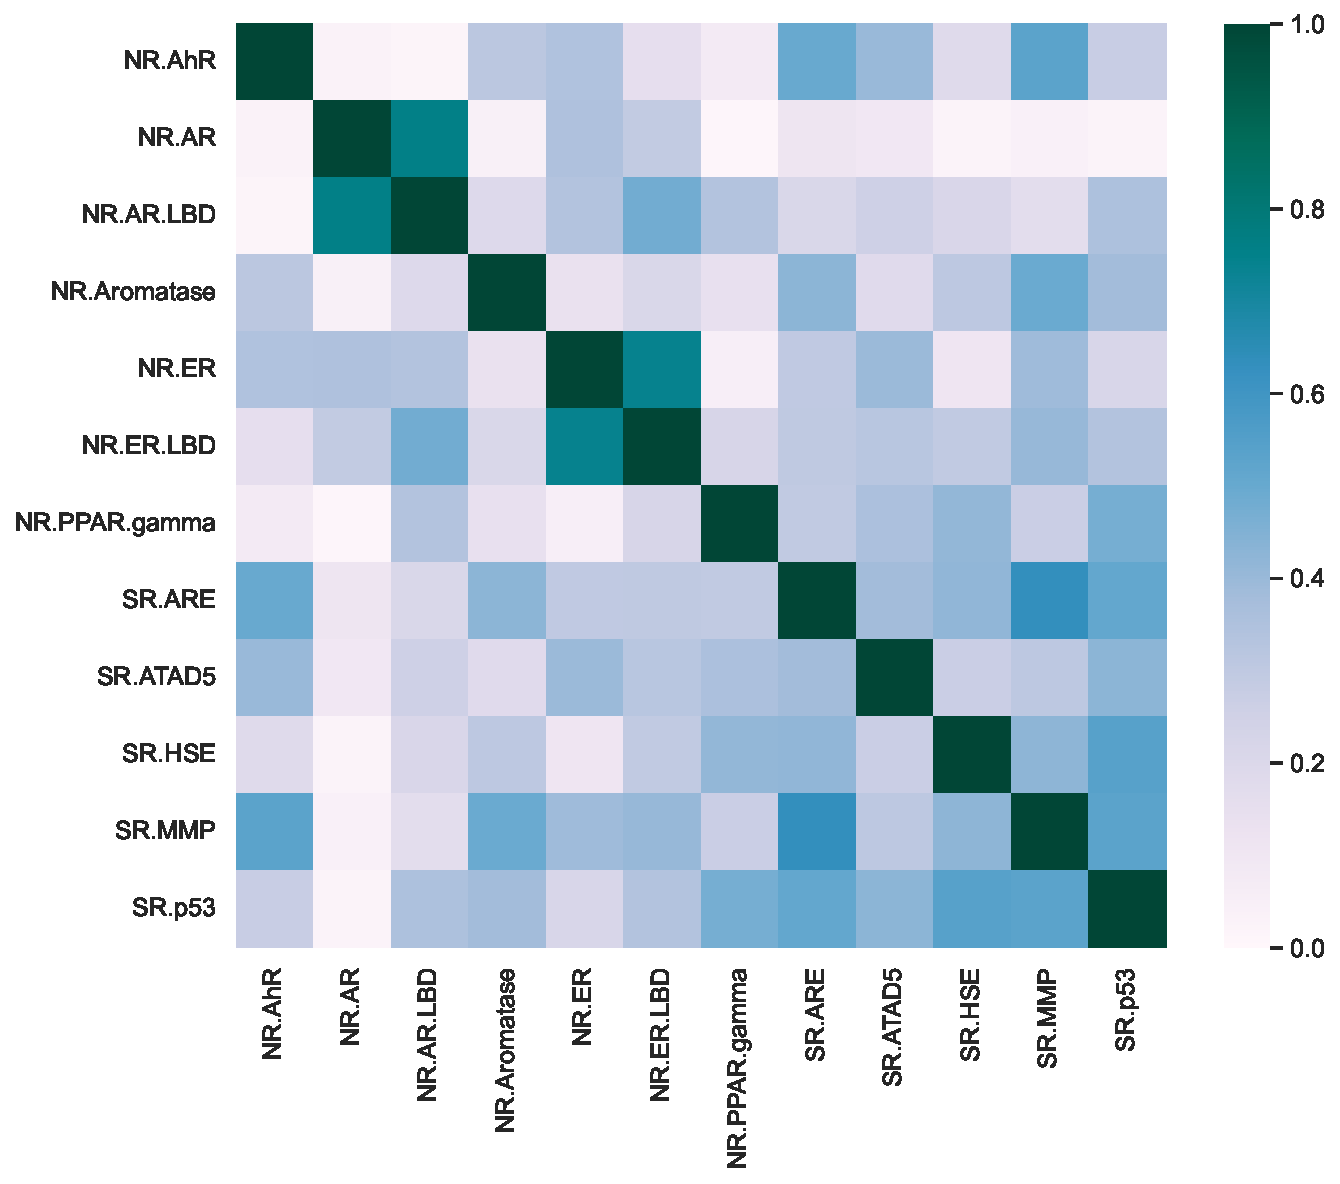
\includegraphics[width=0.6\textwidth]{include/img/appendix/phi_matrix.pdf}
  \caption{Phi coefficient matrix. Phi coefficient measures the association of two binary variables, analogue to the Pearson correlation. It ranges from -1 for high negative association to 1 high positive association. Zero corresponds to no association between the variables. In this matrix, all endpoints had a positive association. }
  \label{fig:phi_coefficient}
\end{figure}

\begin{figure}[h]
	\centering
  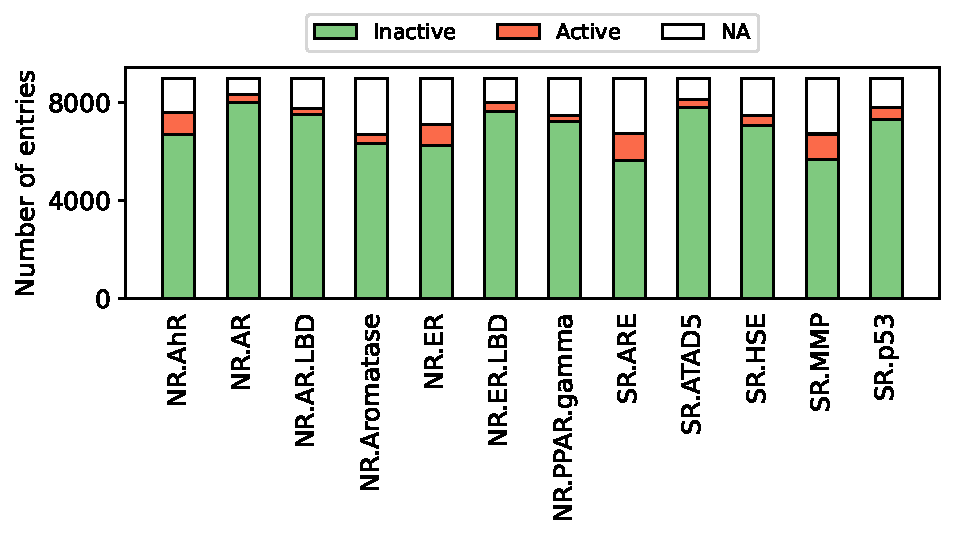
\includegraphics[width=0.8\textwidth]{include/img/results/labelsTox21.pdf}
  \caption{Distribution of endpoint labels in the toxicity dataset. Total number of unique InChIKeys: 8975.}
  \label{fig:bars_endpoints}
\end{figure}	





%###################################################
\phantomsection
\section*{Spectra in MassBank library}
\addcontentsline{toc}{section}{Spectra in MassBank library}

The mass spectra available in MassBank was filtered for the compounds with endpoint labels. The resulting collection included 15808 spectra and 1350 unique InChIKeys, which represents 15\% of the unique InChIKeys in the toxicity dataset. The distribution of the precursors and the number of peaks per spectra are shown in Figure \ref{fig:library}. The average precursor and number of peaks per spectra were 283 \textit{m/z} and 5, respectively.

\begin{figure}[H]
\centering
	 \begin{subfigure}[a]{0.35\textwidth}
 		 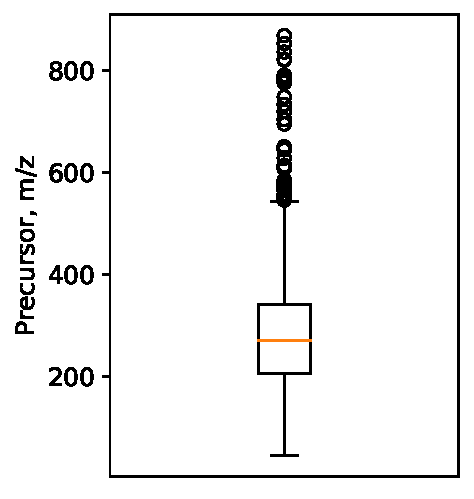
\includegraphics[width=1\textwidth]{include/img/results/Precursors.pdf}
 		 \caption{}
 	\end{subfigure}
 		 \begin{subfigure}[a]{0.35\textwidth}
  		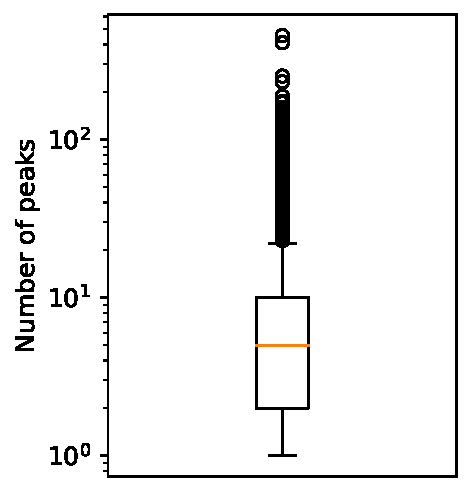
\includegraphics[width=1\textwidth]{include/img/results/NumberPeaks.pdf}
 		 \caption{}
 	\end{subfigure}
\caption{(a) Precursor \textit{m/z} and (b) number of peaks per spectra. The spectra was filtered for the Tox21 Challenge compounds, \tMS{}, and LC-ESI. Number of filtered spectra: 15808. Unique InChIKeys: 1350.}
\label{fig:library}
\end{figure}



%###################################################
\phantomsection
\section*{Mass spectra similarity}
\addcontentsline{toc}{section}{Mass spectra similarity}

The cosine similarity was calculated to compare the combined mass spectra. Very few chemicals scored above 0.7 (139, representing 0.02\% of all pairs) as shown in Figure \ref{fig:frequency_cosine} and Table \ref{table:frequency_cosine}. The distribution of cosine values across the spectra is illustrated in Figure \ref{fig:cosine_ij}. The spectra were ordered using hierarchical clustering that minimizes the variance between all groups at each step of the process. In this way, it is possible to notice regions of high and low similarity on the heatmap. 
\begin{figure}[h]
  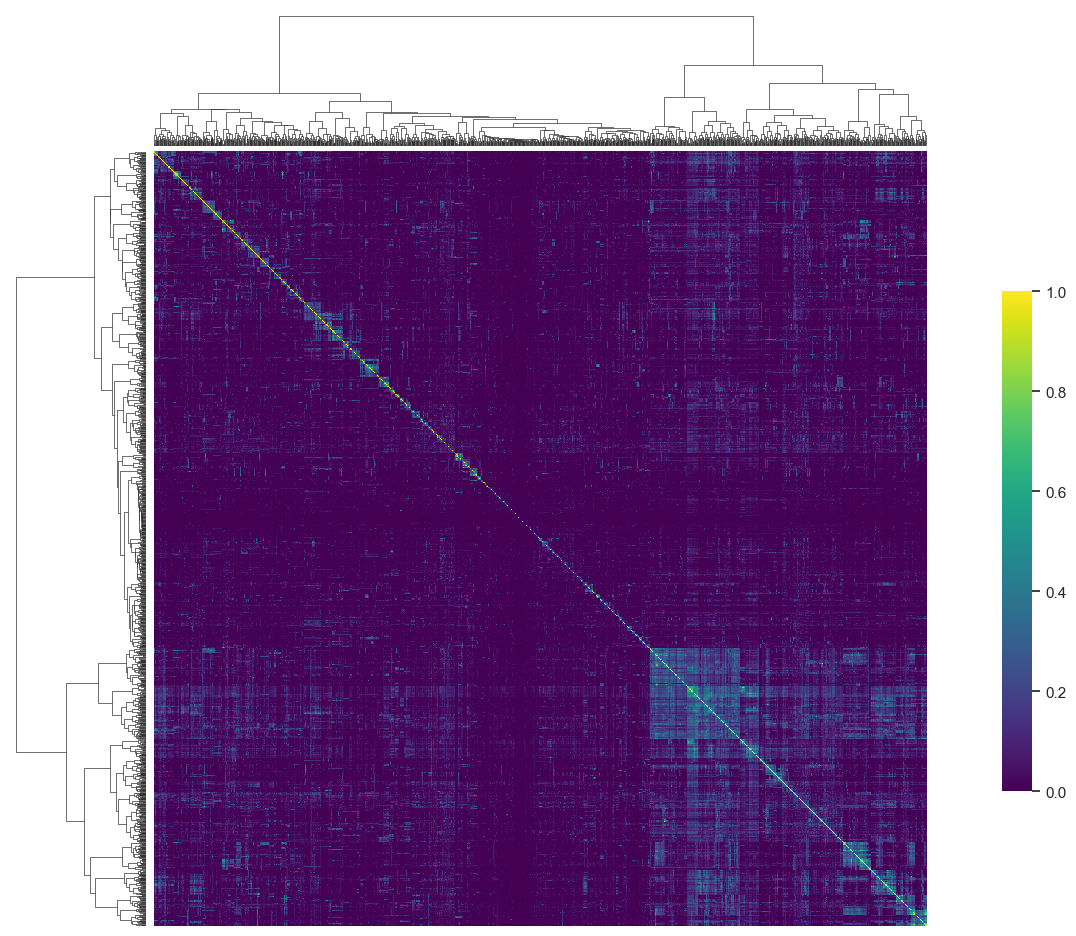
\includegraphics[width=1\textwidth]{include/img/heatmap.png}
  \caption{Cosine similarity heatmap. The x-axis and y-axis of the heatmap includes the combined mass spectra for unique InChIKeys ordered by hierarchical clustering. The hierarchical distribution allows to visualize groups with similar spectra. Green zones of high similarity (lower right corner and small groups across the diagonal) suggest groups of chemical classes, while purple areas indicate low similarity and no groups. The diagonal is the cosine similarity for the same spectra and it is 1. }
  \label{fig:cosine}
\end{figure}

\clearpage
\begin{figure}[h]
  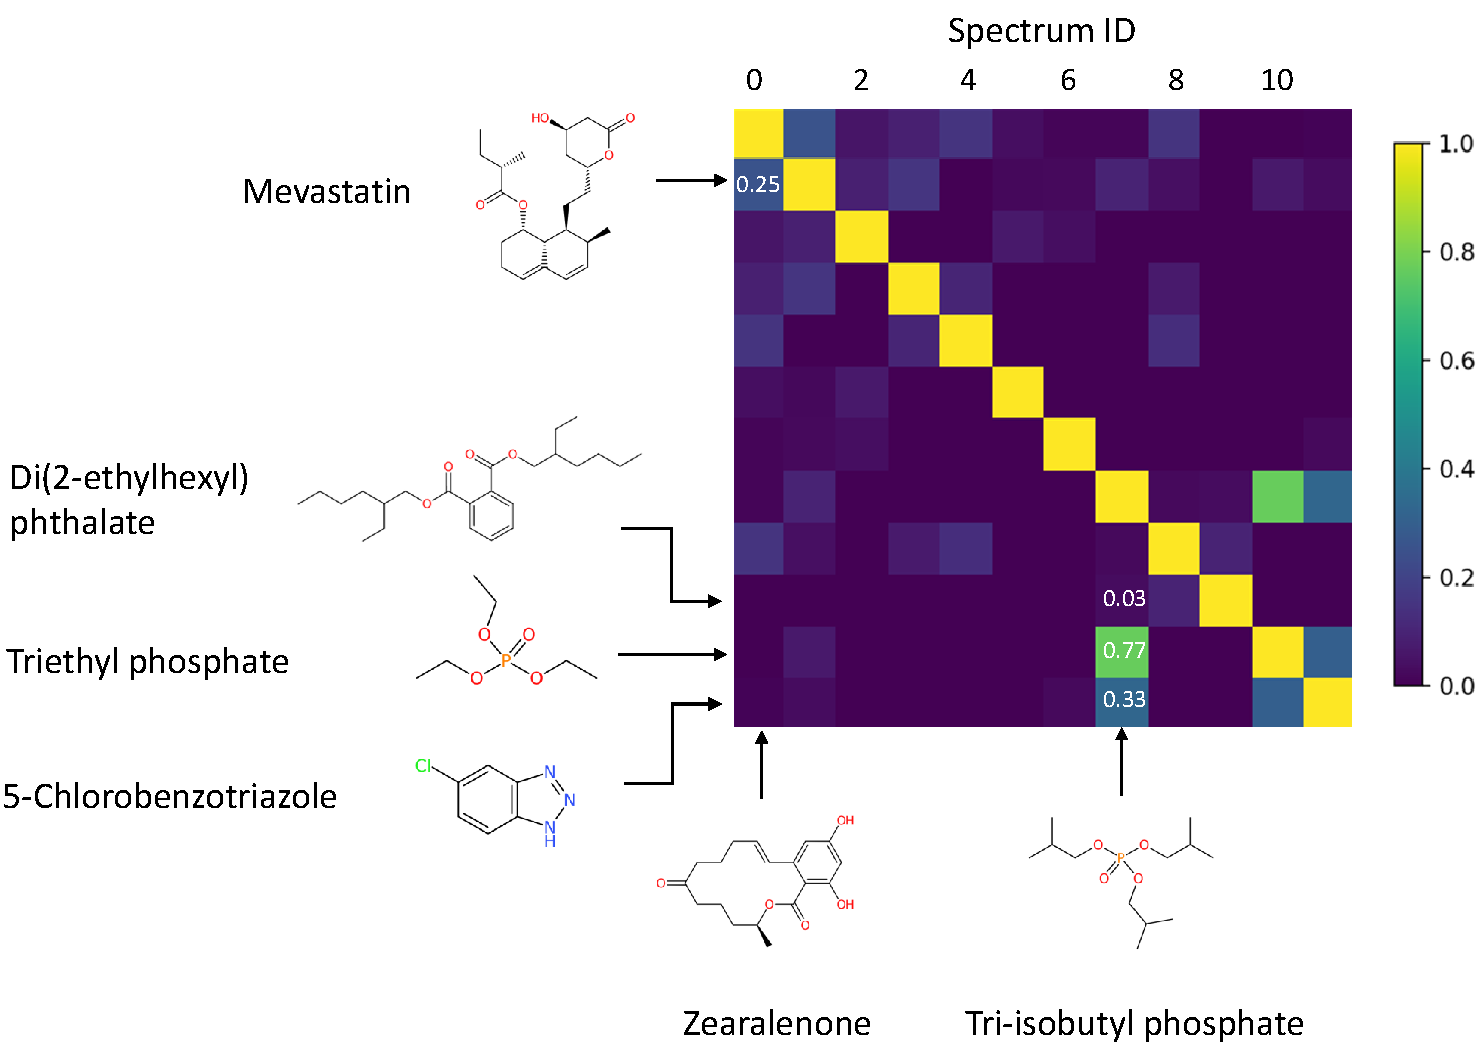
\includegraphics[width=1\textwidth]{include/img/results/cosine_zoom_in.pdf}
  \caption{Cosine similarity matrix for a subset of mass spectra. The cosine score is high for the phosphate pair, while low for zearalenone in the subset indicating favorable selectivity of the cosine score. Additional pairs with cosine score greater than 0.6 are illustrated with their chemical structures in Figure \ref{fig:net_structures}. The diagonal is the cosine similarity for the same spectra. }
  \label{fig:cosine_zoomed_in}
\end{figure}


\begin{figure}[h]
    \centering
	 \begin{subfigure}[b]{0.48\textwidth}
 		 \hspace{3cm} 
 		 \centering
 		 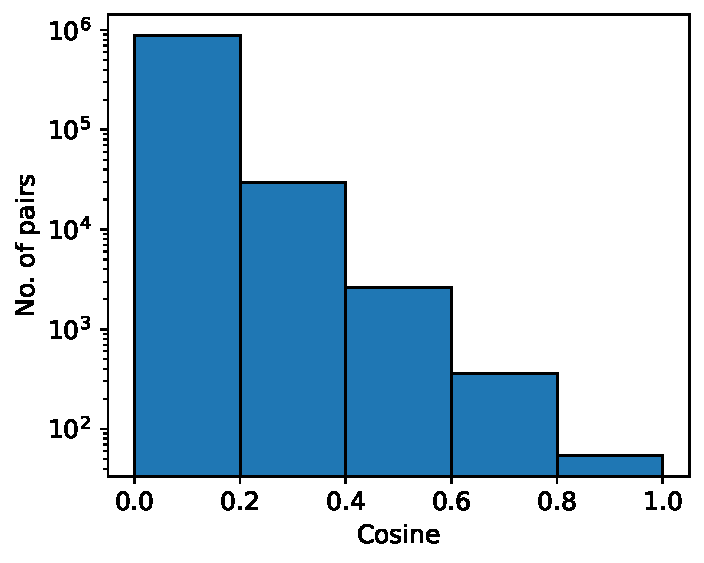
\includegraphics[width=1\textwidth]{include/img/results/cosine_pairs_log.pdf}
 		 \caption{}
 	\end{subfigure}
 	\hfill
 		 \begin{subfigure}[b]{0.48\textwidth}
 		 \hspace{3cm}
 		 \centering
  		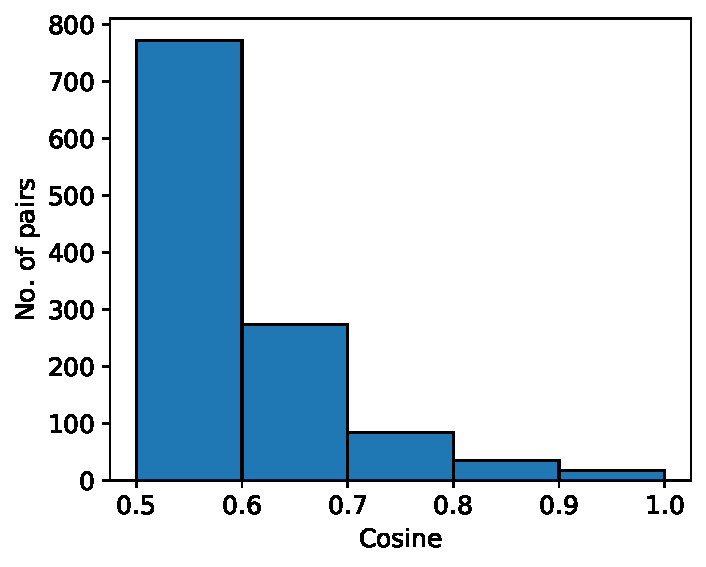
\includegraphics[width=1\textwidth]{include/img/results/cosine_pairs_05.pdf}
 		 \caption{}
 	\end{subfigure}
  \caption{(a) Absolute frequency for all cosine scores and (b) for cosine scores greater than 0.5. Cosine is calculated for all pairs in the processed dataset with tolerance 0.1 \textit{m/z}.}
  \label{fig:frequency_cosine}
\end{figure}

The cosine similarity of a subset of mass spectra is shown on Figure \ref{fig:cosine_zoomed_in}. It can be seen that the cosine score is high for the pair of phosphates, correctly reflecting their structural similarity. Conversely, zearalenone (first column from the left) exhibits low cosine similarities, indicating a favorable selectivity of the cosine score for these pairs.

The relationship between the cosine and the number of matched peaks in the combined spectra is shown in Figure \ref{fig:cosine_ij}. The number of matched peaks corresponds to the number of common peaks within a tolerance of 0.1 \textit{m/z}. The figure shows a low density in the high cosine range over 0.7. 



\begin{figure}[h]
\centering
  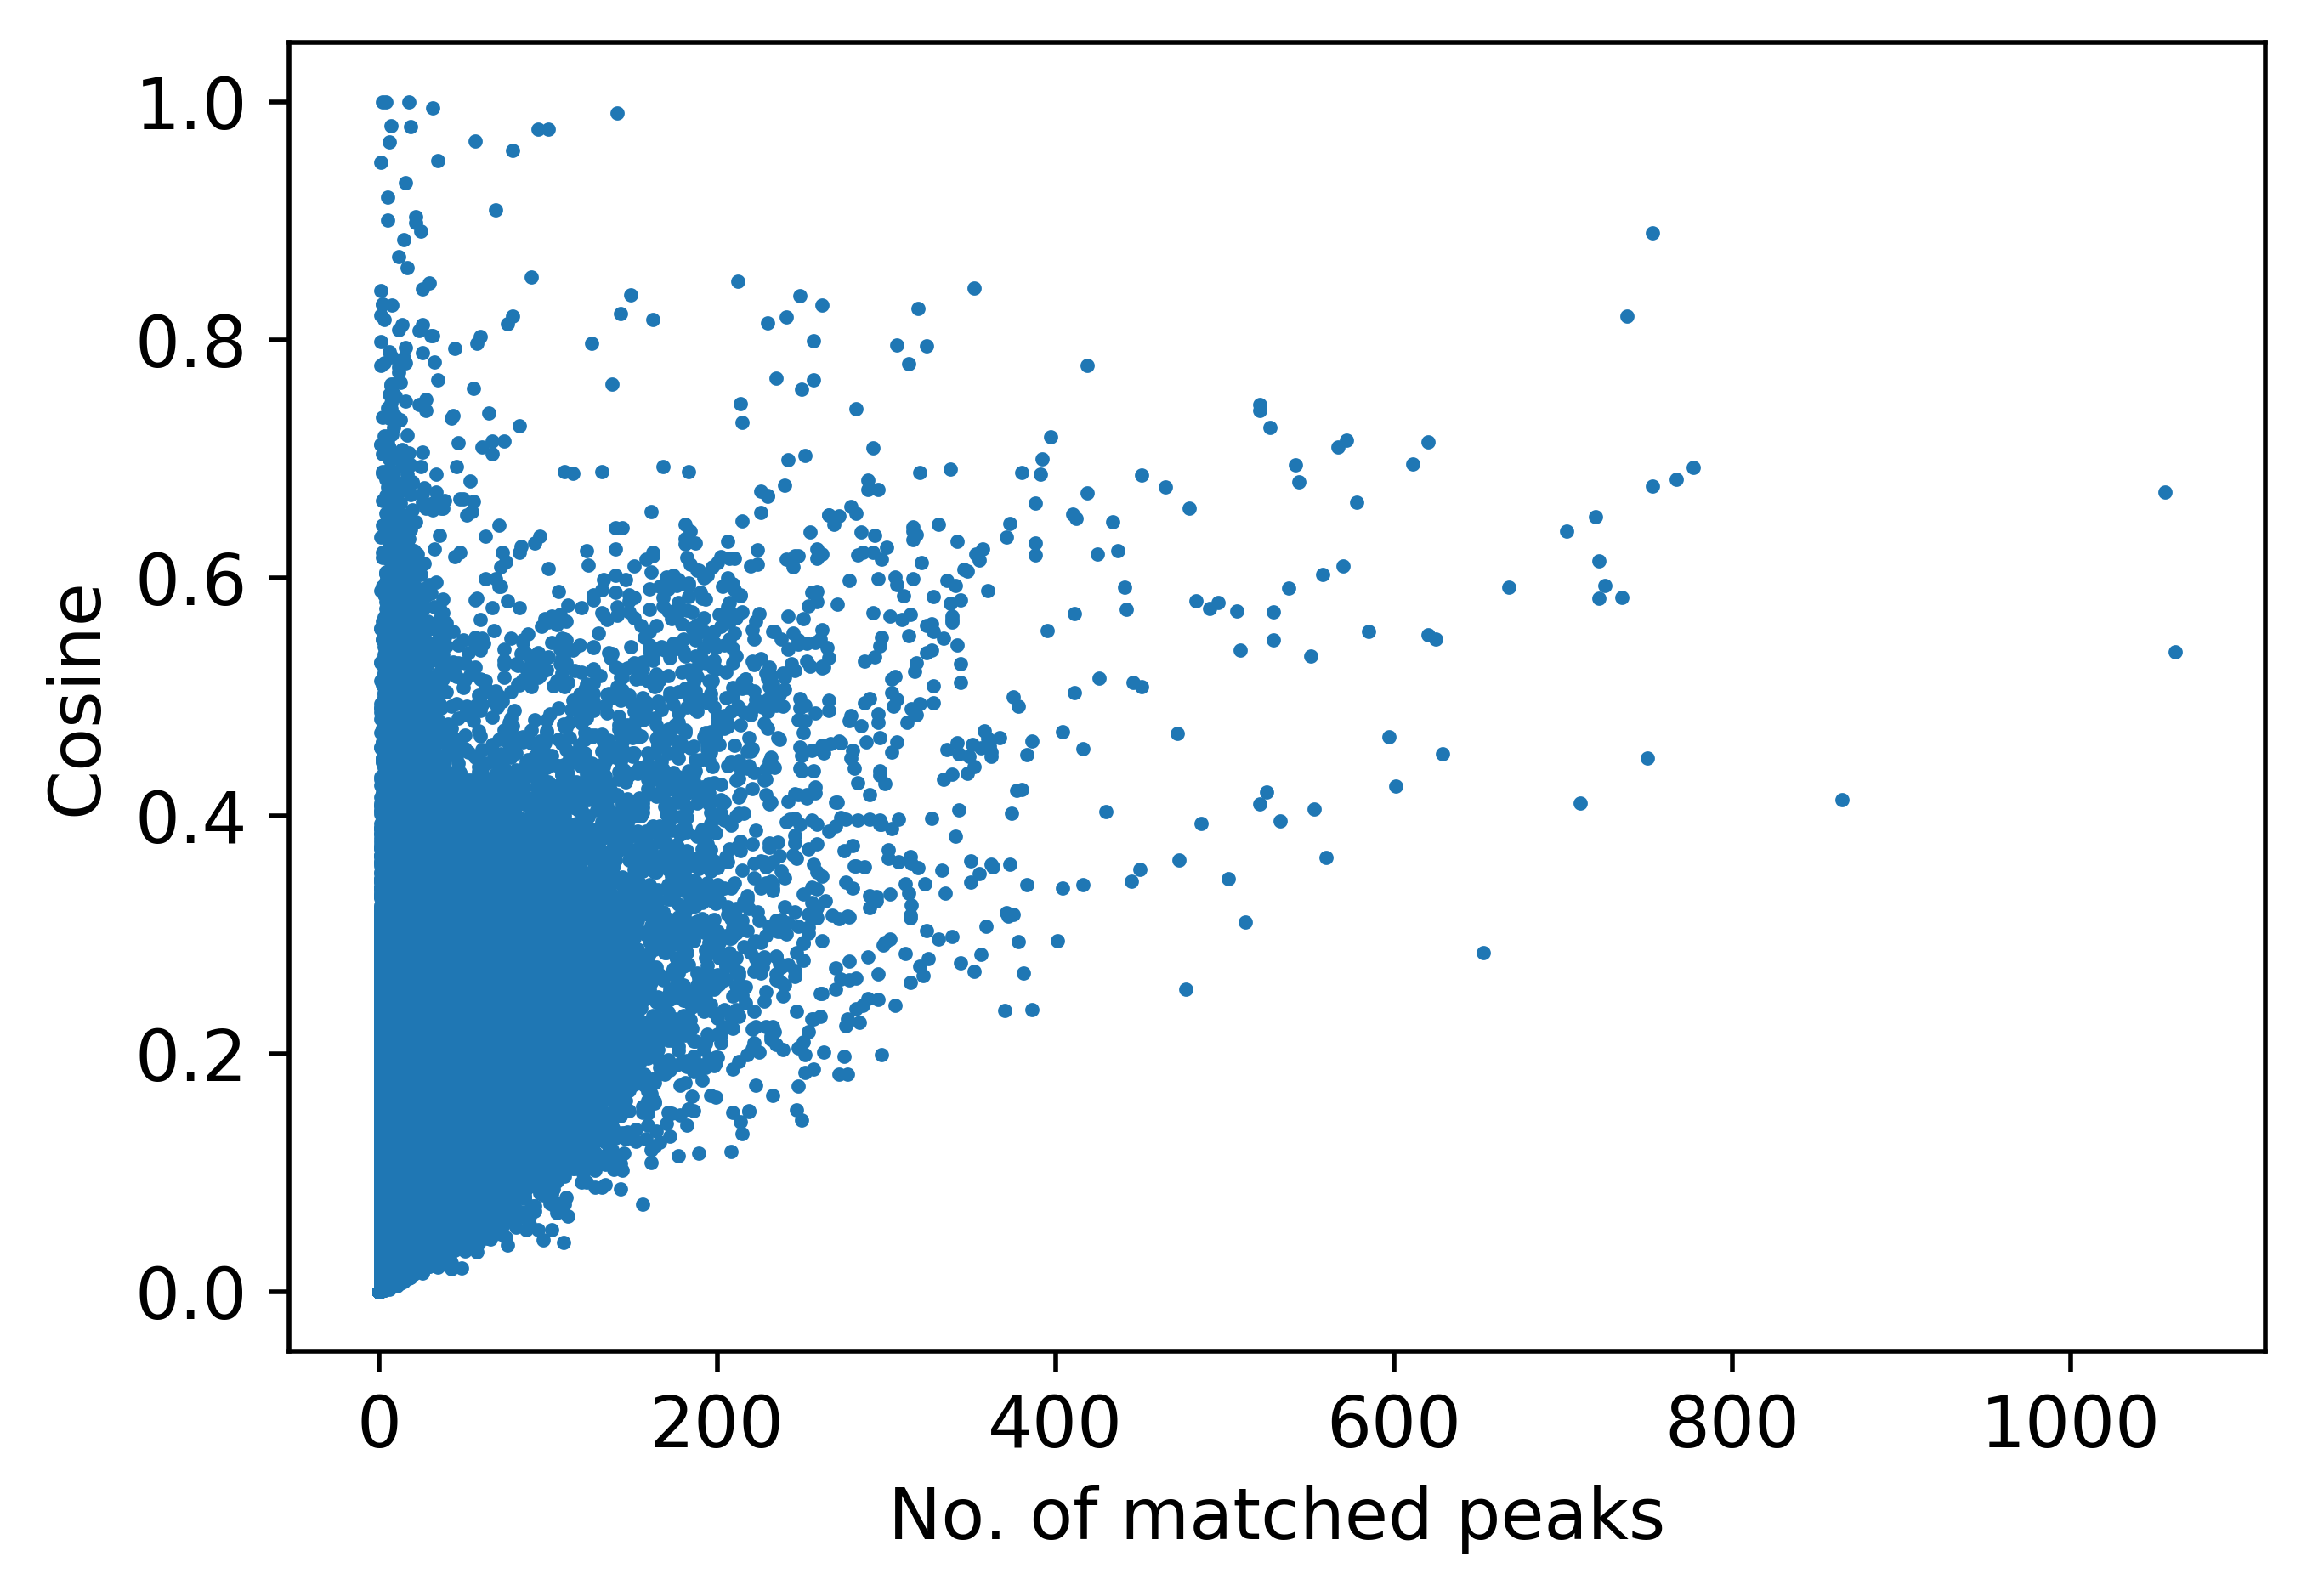
\includegraphics[width=0.8\textwidth]{include/img/results/cosine_ij.png}
  \caption{Relationship between the cosine score and the number of matched peaks in the combined spectra. A combined spectra contains all the peaks from library spectra having the same InChIKey. A peak from the combined spectra A is matched with a peak from the combined spectra B if the second lies within a tolerance of 0.1 \textit{m/z}. Each peak can only be matched once. The figure shows a high-density area in the lower-left part and low density in the upper part. The latter depicts pairs of spectra that can form the spectral networks. High and atypical values are further discussed.}
  \label{fig:cosine_ij}
\end{figure}

%###################################################
\clearpage
\phantomsection
\section*{Spectral similarity networks}
\addcontentsline{toc}{section}{Spectral similarity networks}
\label{sec:networks}

The cosine similarity was used to build the network. Several parameters were tested including the tolerance for the cosine calculation, minimum score, and maximum edges from a node, as described in Table \ref{table:nets_opt}. Then, a network was selected considering the number of nodes, edges, other network statistics, and visual inspection. The final network had 363 nodes, 409 edges and 105 connected components. The statistics summary for the selected network is shown in column ``cosine'' in Table \ref{table:cos_M2DS_networks_parameters}. Additionally, the same table includes the statistics for an experimental network based on a machine learning similarity metric. These two networks share similar clustering coefficient, network density, and connected components. Not remarkable differences were observed for the distribution of the endpoint labels compared to cosine similarity for the studied collection of spectra. The MS2DeepScore shows great promise for spectra clustering, a network is examplified for the endpoints NR.AR and SR.ARE in Figure \ref{fig:MS2DS_networks}.

The distribution of endpoints for the endpoint NR.AR and SR.ARE is shown in Figure \ref{fig:networks}. The NR.AR is a representative case of an endpoint that showed clustering tendency, while the SR.ARE represents low clustering tendency with active labels distributed across different clusters. All endpoint labels distribution is illustrated in the figures of Appendix \ref{appendix:networks}.


\begin{table}[h]
\centering
\footnotesize
\csvautobooklongtable[table head=\caption{Summary of conditions and statistics of the cosine similarity network and a network based on a deep learning-based score.}\label{table:cos_M2DS_networks_parameters}\\\hline
               \csvlinetotablerow\\\hline
               \endfirsthead\hline
               \csvlinetotablerow\\\hline
               \endhead\hline
               \endfoot]{include/tables/networks_parameters.csv}
\caption*{Note: The second column is the selected network for further processing and predictions. The third column is an example of a network built with MS2DeepScore. The statistics were obtained in Cytoscape.}
\end{table}


\begin{figure}[H]
  \centering
	 \begin{subfigure}[a]{1\textwidth}
 		 \centering
  		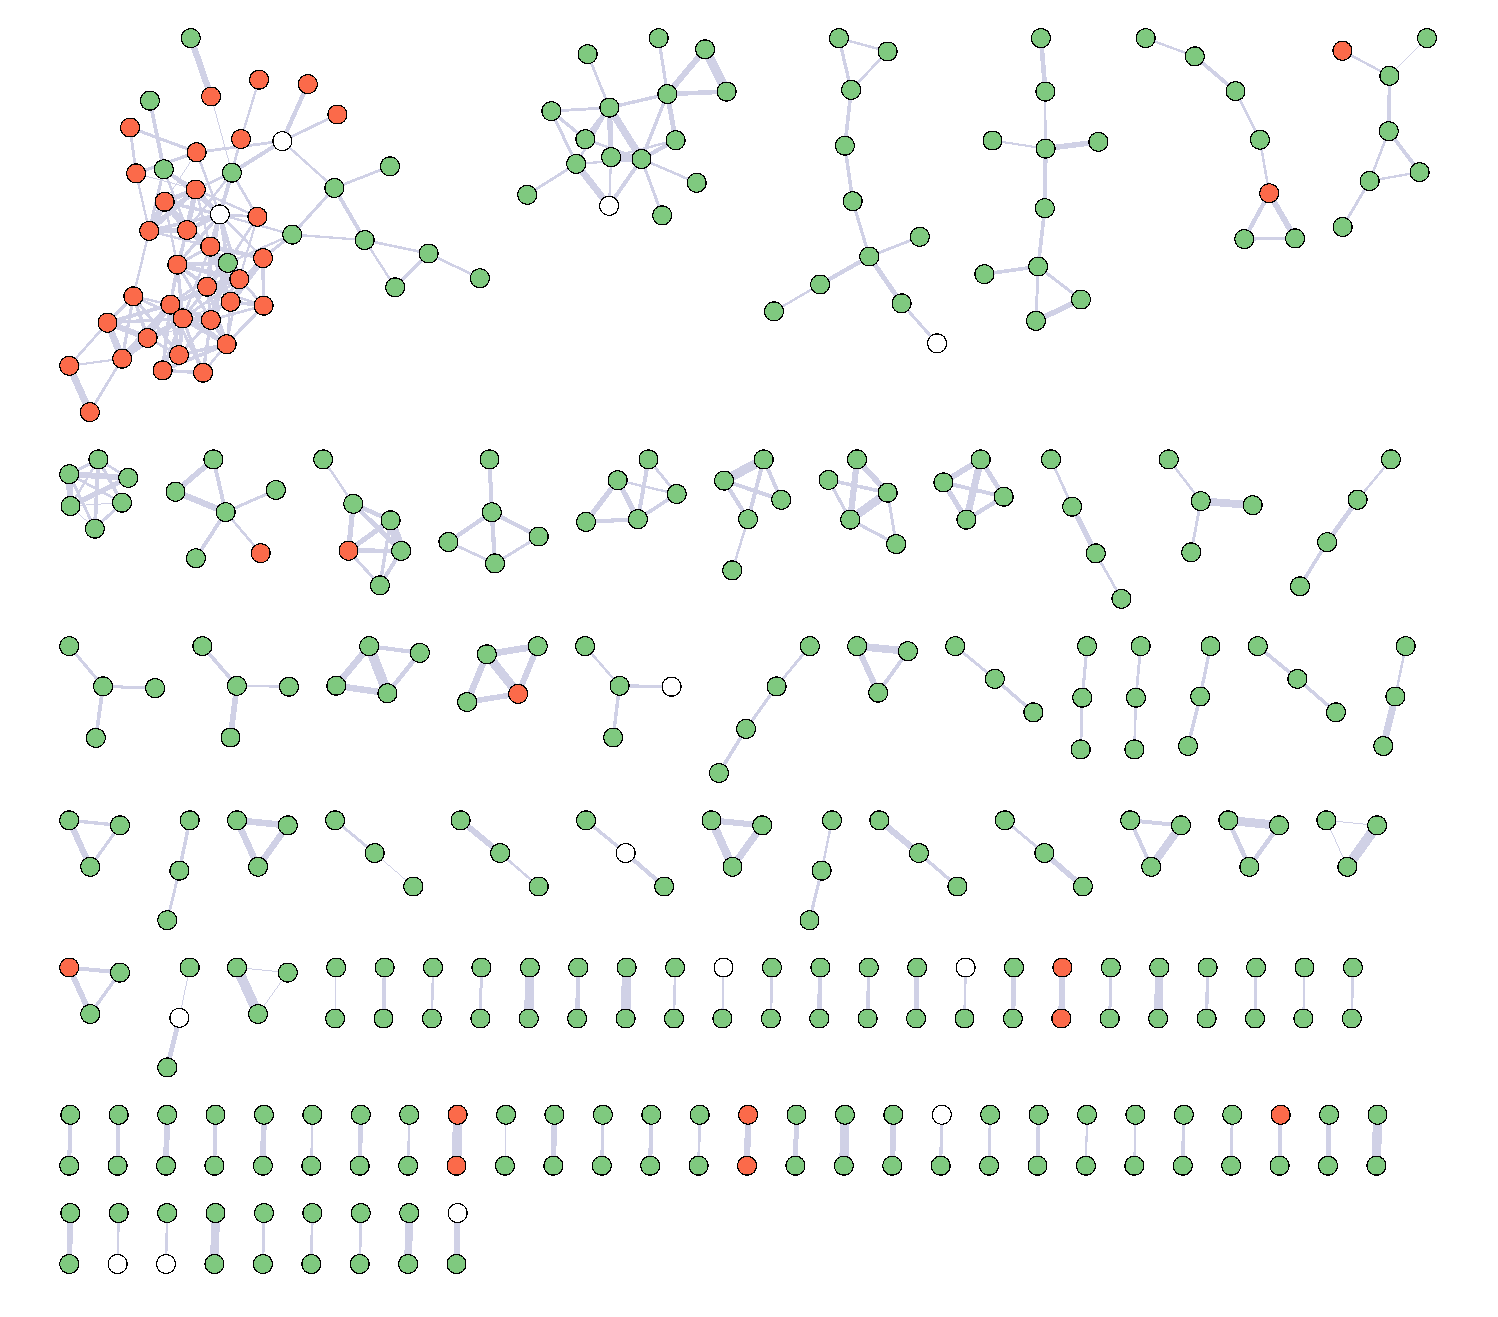
\includegraphics[width=0.7\textwidth]{include/img/appendix/nets_endpoints/NR.AR.pdf}
 		 \caption{}
 	\end{subfigure}
 	\hfill
 		 \begin{subfigure}[a]{1\textwidth}
 		 \centering
 		 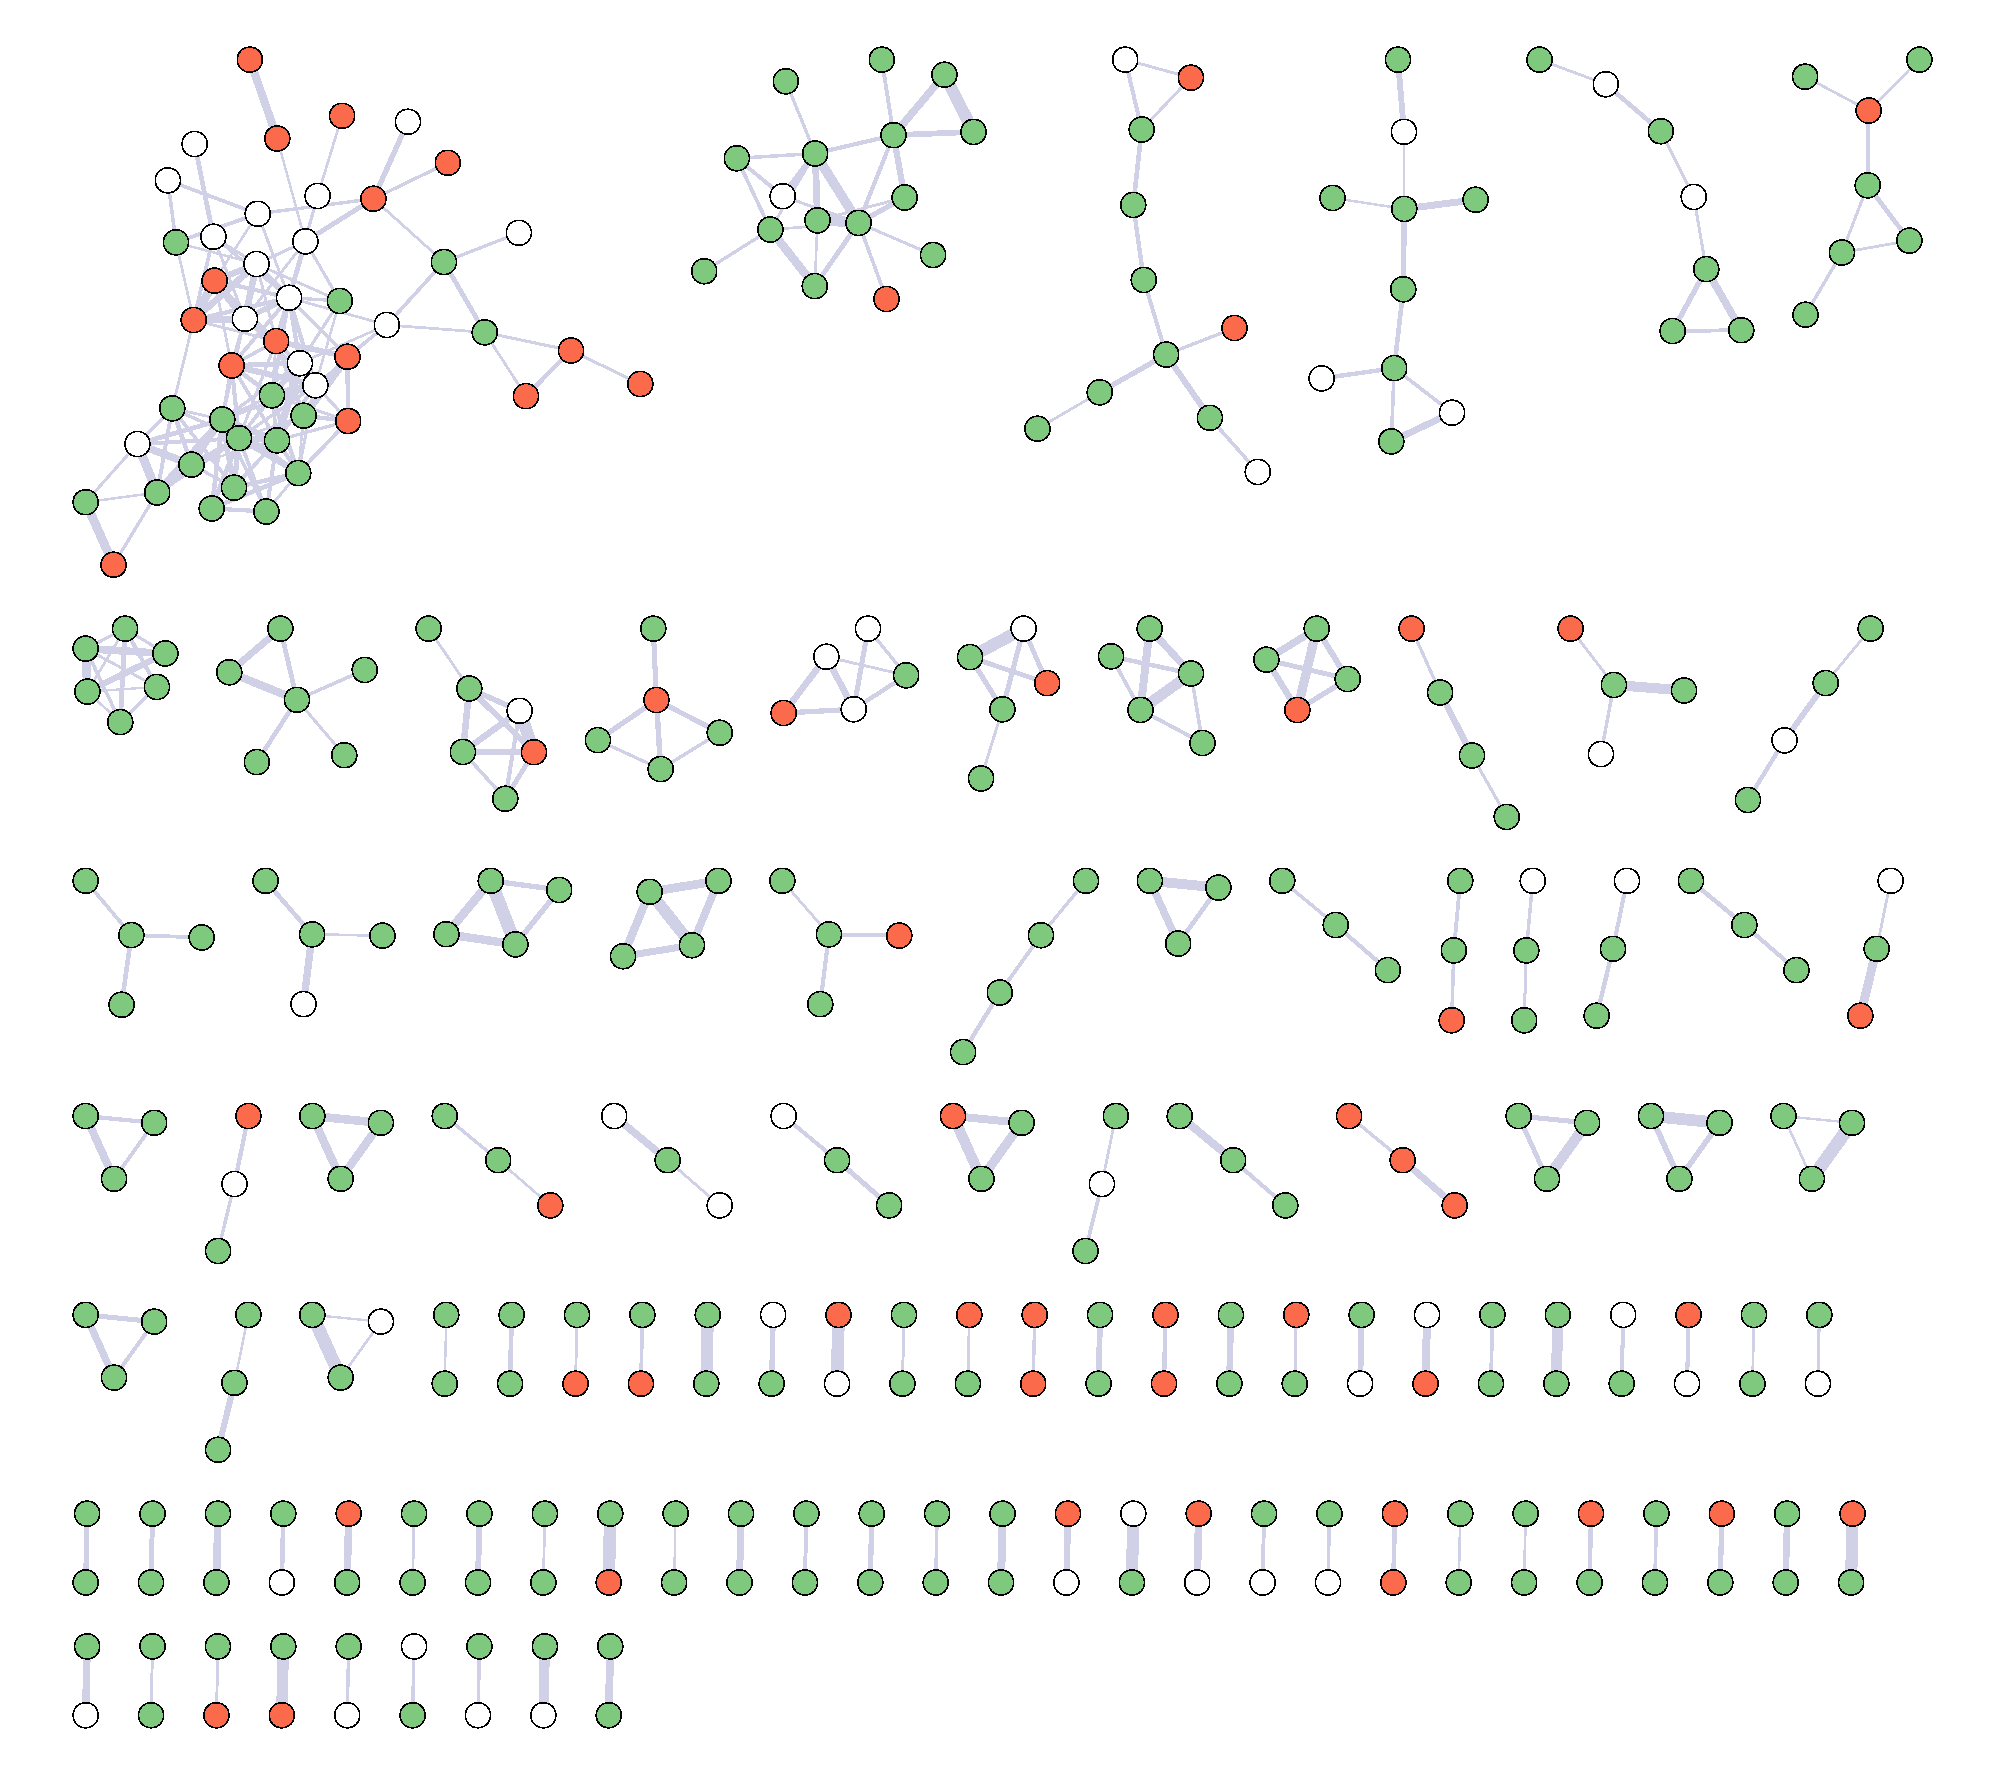
\includegraphics[width=0.7\textwidth]{include/img/appendix/nets_endpoints/SR.ARE.pdf}
 		 \caption{}
 	\end{subfigure}
  \caption{Spectral similarity network for the endpoint (a) NR.AR and (b) SR.ARE. Minimum cosine score: 0.6. Active endpoints are in red, inactive in green, and blank if the a label was not available. The nodes represent the combined mass spectra of unique chemicals. The edge width indicates the intensity of the cosine similarity. The spectral similarity networks for all the endpoint labels are shown in Appendix \ref{appendix:networks}.}
  \label{fig:networks}
\end{figure}






%###################################################
\phantomsection
\section*{\textit{k}-NN algorithm}
\addcontentsline{toc}{section}{\textit{k}-NN algorithm}

Two approaches for the prediction of the endpoints were tested: \textit{k}-NN and spectral similarity networks. {k}-NN algorithm explored the entire dataset and assigned a label based on the \textit{k} nearest neighbors according to their cosine similarity. On the other hand, the spectral similarity network narrowed the chemical space and pre-defined the neighbors for a chemical based on, among other factors, a cosine similarity threshold. 

The {k}-NN algorithm requires the definition of two hyperparameters, the distance metric and \textit{k}. The distance parameter was the cosine distance. The best \textit{k} was determined by cross-validation. The change of recall for different values of \textit{k} for NR.AR and NR.AhR is shown Figure \ref{fig:k_values}. In the case of NR.AR, the recall was stable for the explored values of \textit{k}, but for the rest of endpoints the recall decreased with the increase of \textit{k} as illustrated with NR.AhR.

\begin{table}[h]
\centering
\footnotesize
\csvautobooklongtable[
			table head=\caption{Recall and precision for \textit{k}-NN}\label{table:kNN_metrics}\\\hline
               \csvlinetotablerow\\\hline
               \endfirsthead\hline
               \csvlinetotablerow\\\hline
               \endhead\hline
               \endfoot,
			respect all]{include/tables/kNN_metrics.csv}
\caption*{Note: The recall and precision were calculated based on a stratified test set (20\%) of the entire dataset. Number of samples: 1350. The active and inactive columns are the number of compounds with the respective labels in the toxicity data.}
\end{table}



%Moved

%###################################################
%\newpage
\clearpage
\phantomsection
\section*{\textit{k}-NN algorithm in locally connected mass spectra}
\addcontentsline{toc}{section}{\textit{k}-NN algorithm in locally connected spectra}

After building the network, its prediction ability was tested. A representation of the chemical class of the nodes, the predicted and true labels are illustrated in Figure \ref{fig:NR.AR_class}. Recall and precision were estimated by leave-one-out and they are shown in Table \ref{table:metrics_knet}.  The highest recall and precision were obtained for NR.AR, being 81.8\% and 75.0\%, respectively; and the lowest for SR.HSE, being 15.8\% and 13.0\%. The same table also shows the number of labels for each endpoint. The active/inactive ratio range was between 27.3\% for SR.ARE and 2.9\% for NR.PPAR.gamma.

The network was used for the retrospective analysis of a wastewater sample from an effluent of a treatment plant. Some features of the real sample show similarity with the nodes in the reference network. The reference network and the \tMS{} features of the sample are displayed in Figure \ref{fig:sample}.

\begin{table}[h]
\centering
\footnotesize
\csvautobooklongtable[table head=\caption{Recall and precision for the \textit{k}-NN based on locally connected nodes within a spectral network}\label{table:metrics_knet}\\\hline
               \csvlinetotablerow\\\hline
               \endfirsthead\hline
               \csvlinetotablerow\\\hline
               \endhead\hline
               \endfoot,
			respect all]{include/tables/metrics_knet.csv}
\caption*{Note: The recall and precision were estimated based on leave-one-out over the entire network. Number of nodes: 363. The active and inactive columns are the number of compounds with the respective labels in the toxicity data.}
\end{table}

\begin{figure}
  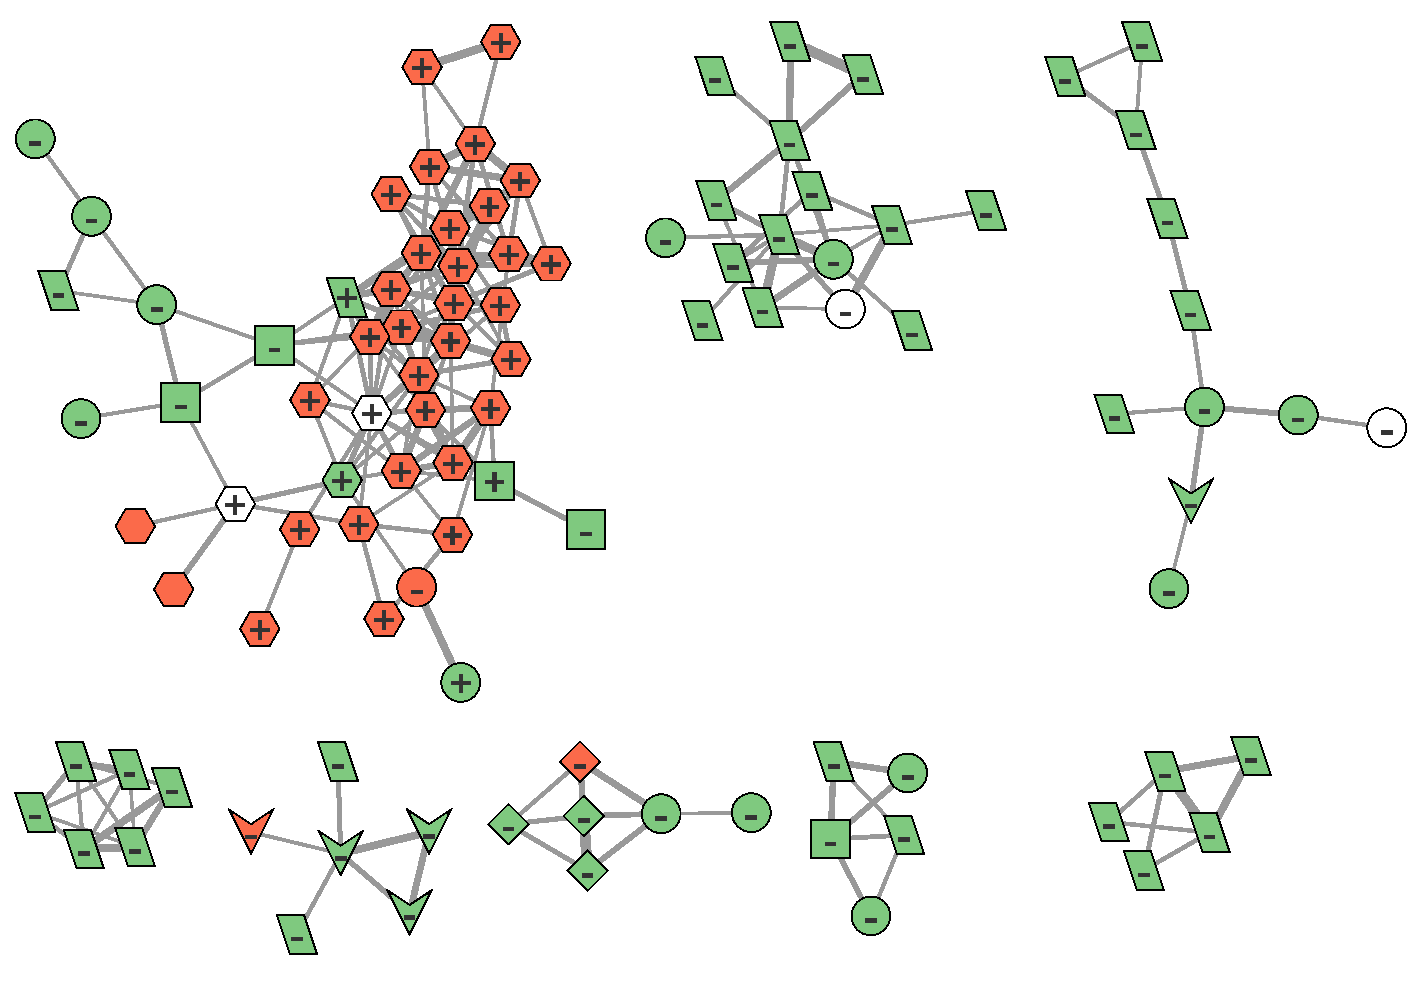
\includegraphics[width=1\textwidth]{include/img/results/NR.AR_class.pdf}
  \caption{Predicted and true labels for the NR.AR endpoint on a subset of nodes. The nodes represent mass spectra, the fill color indicates the true labels as active (in red), inactive (in green) or not available (in white). The symbols inside the nodes show the predicted labels as active (+) or inactive (-). The edge width illustrates the intensity of the spectral similarity. The shape of the node corresponds to the chemical class according to ChemOnt obtained from ClassyFire \cite{DjoumbouFeunang2016}. Hexagon: steroids and steroid derivatives. Diamond: phenols. Parallelogram: benzene and substituted derivatives. Rectangle: prenol lipids. V: Organic phosphoric acids and derivatives. Circle: other classes.}
  \label{fig:NR.AR_class}
\end{figure}



\begin{sidewaysfigure}
\centering
  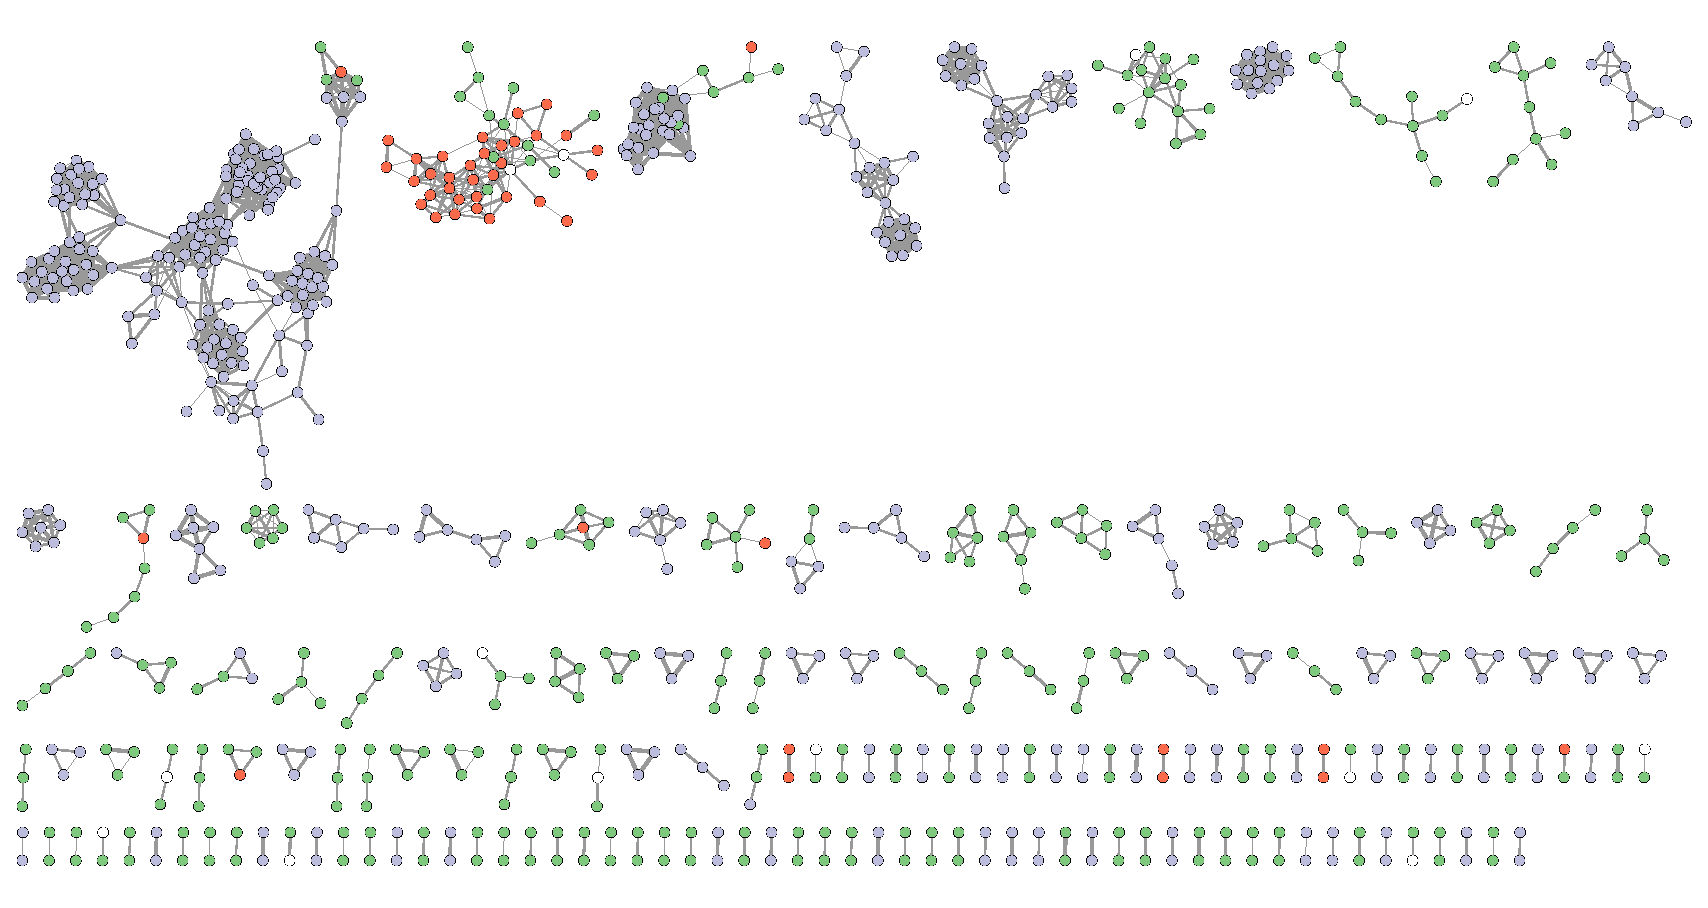
\includegraphics[width=1\textwidth]{include/img/appendix/sample/DDApos.pdf}
  \caption{Toxicity network for the NR.AR endpoint and unknown chromatographic \tMS{} features from a wastewater sample. The active compounds are in red, inactive in green, and detected \tMS{} features in light purple. Nodes without color do not have a NR.AR label in the toxicity dataset. The graph shows independent clusters suggesting, in most cases, low similarity between the reference and sample spectra, and reduced overlap with the chemical space of the toxicity dataset.}
  \label{fig:sample}
\end{sidewaysfigure}

%###################################################


\phantomsection
\section*{Retrospective analysis of \tMS{} features}
\addcontentsline{toc}{section}{Retrospective analysis of \tMS{} features}

The \tMS{} features of a wastewater sample were analyzed using the spectra similarity network for the prediction of NR.AR activity. The sample exhibited multiple dense clusters of spectra with limited connections to the toxicity network, as depicted in Figure \ref{fig:sample}.

Mass spectra features were screened based on their connectivity to active spectra in the spectral network. A few mass spectra features were found to have connections with the reference network. When compared to the reference network, the sample features displayed low cosine similarities. Examples of spectra comparison for features and nodes are shown below. Certain sample spectra exhibited low number of matched peaks, as illustrated in Figure \ref{fig:sample_spectra} (3 peaks) and \ref{fig:sample_spectra_bufexamac} (3 peaks), while others had a higher number of matched peaks, as exemplified in Figure \ref{fig:spectra_sample_steroid} (82 peaks). Even with high number of matched peaks, the cosine similarity score can be low for reference spectra containing a high number of peaks.

To establish node connections, an alternative approach involves considering the common peaks, such as directly by the number of matched peaks or by incorporating weights. The number of matched peaks can provide useful information to describe the connections. By considering the number of matched peaks and lowering the minimum cosine score, an edge can be established between each sample feature and the network. Subsequently, the endocrine disruptive label is assigned based on the votes from connected nodes. For example, the feature of Figure  \ref{fig:spectra_sample_steroid} is connected to 8 active and 1 inactive nodes, then this feature can be predicted as active for NR.AR. This method allows for determining the relatedness of each feature to the nodes in the reference network and identifying those with a higher number of common peaks with active nodes. Consequently, the identified compounds with positive predicted activity can be prioritized for further investigations.

\begin{figure}[h]
  \centering
  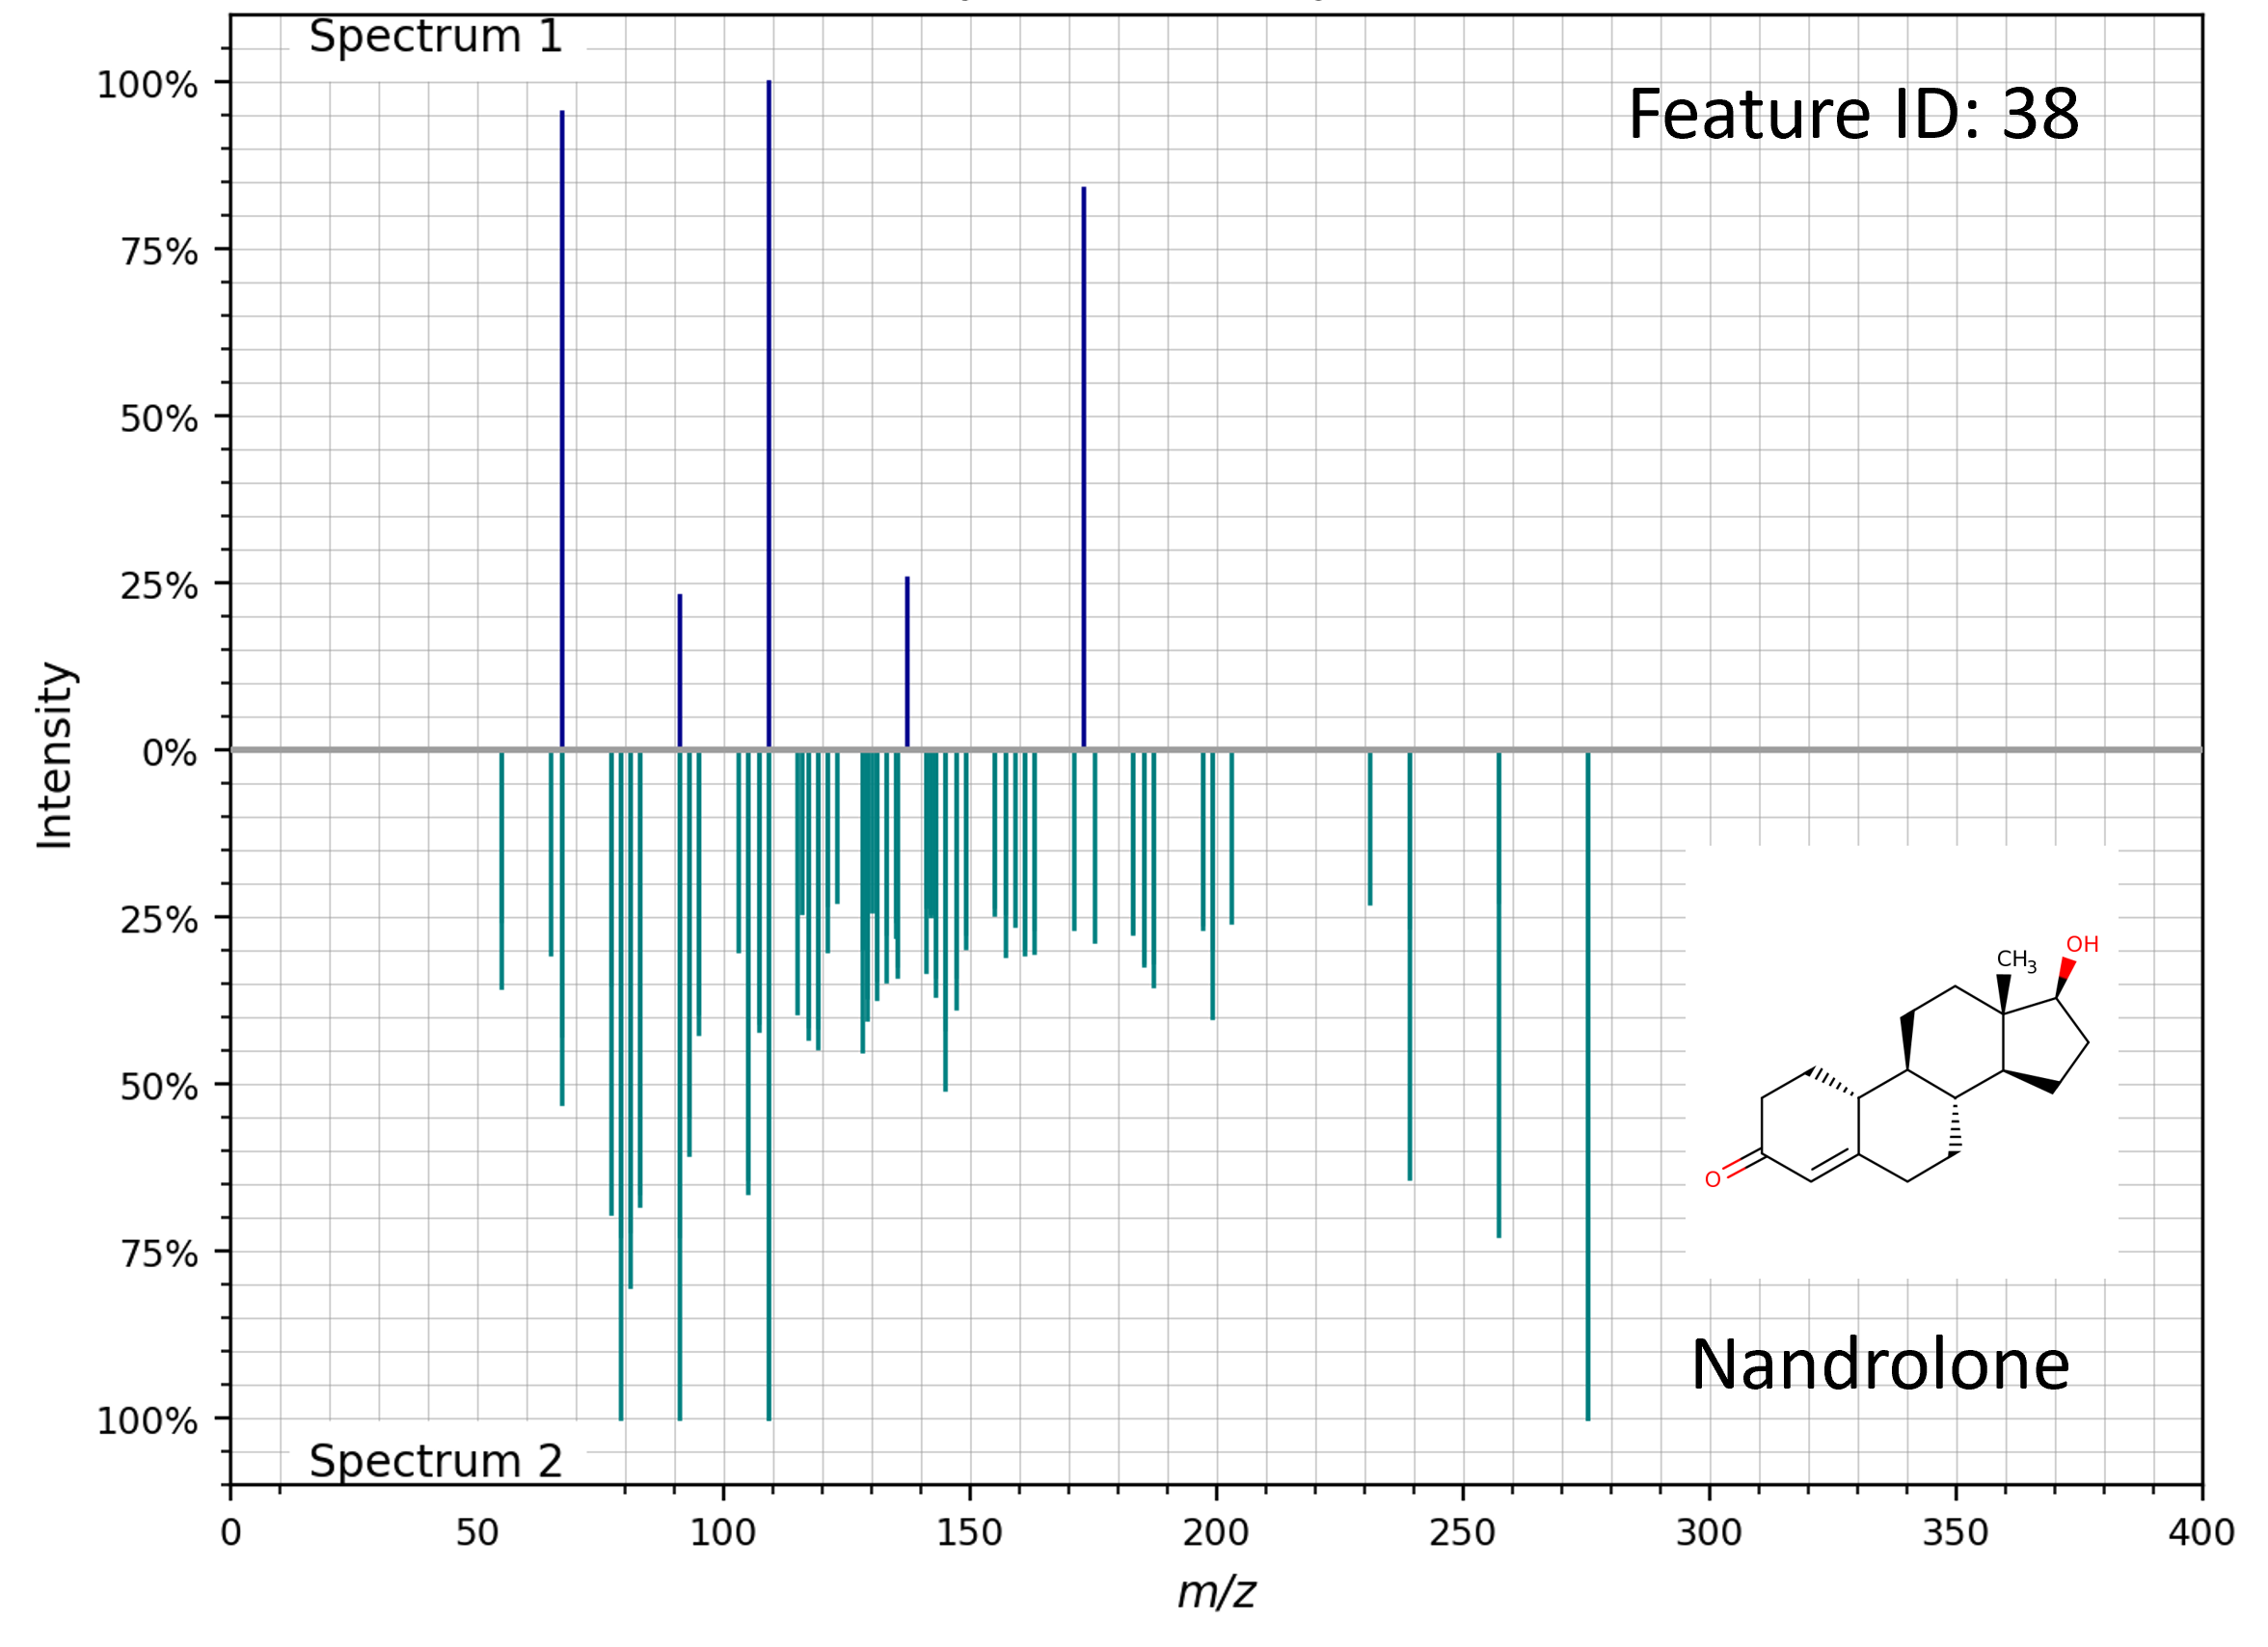
\includegraphics[width=0.8\textwidth]{include/img/appendix/sample/spectra_sample.png}
  \caption{Comparison of a sample feature with a reference spectra (nandrolone: active for NR.AR). The figure exemplifies the cases in which there are a high number of peaks for the reference node.}
  \label{fig:sample_spectra}
\end{figure}


\begin{figure}[h]
  \centering
  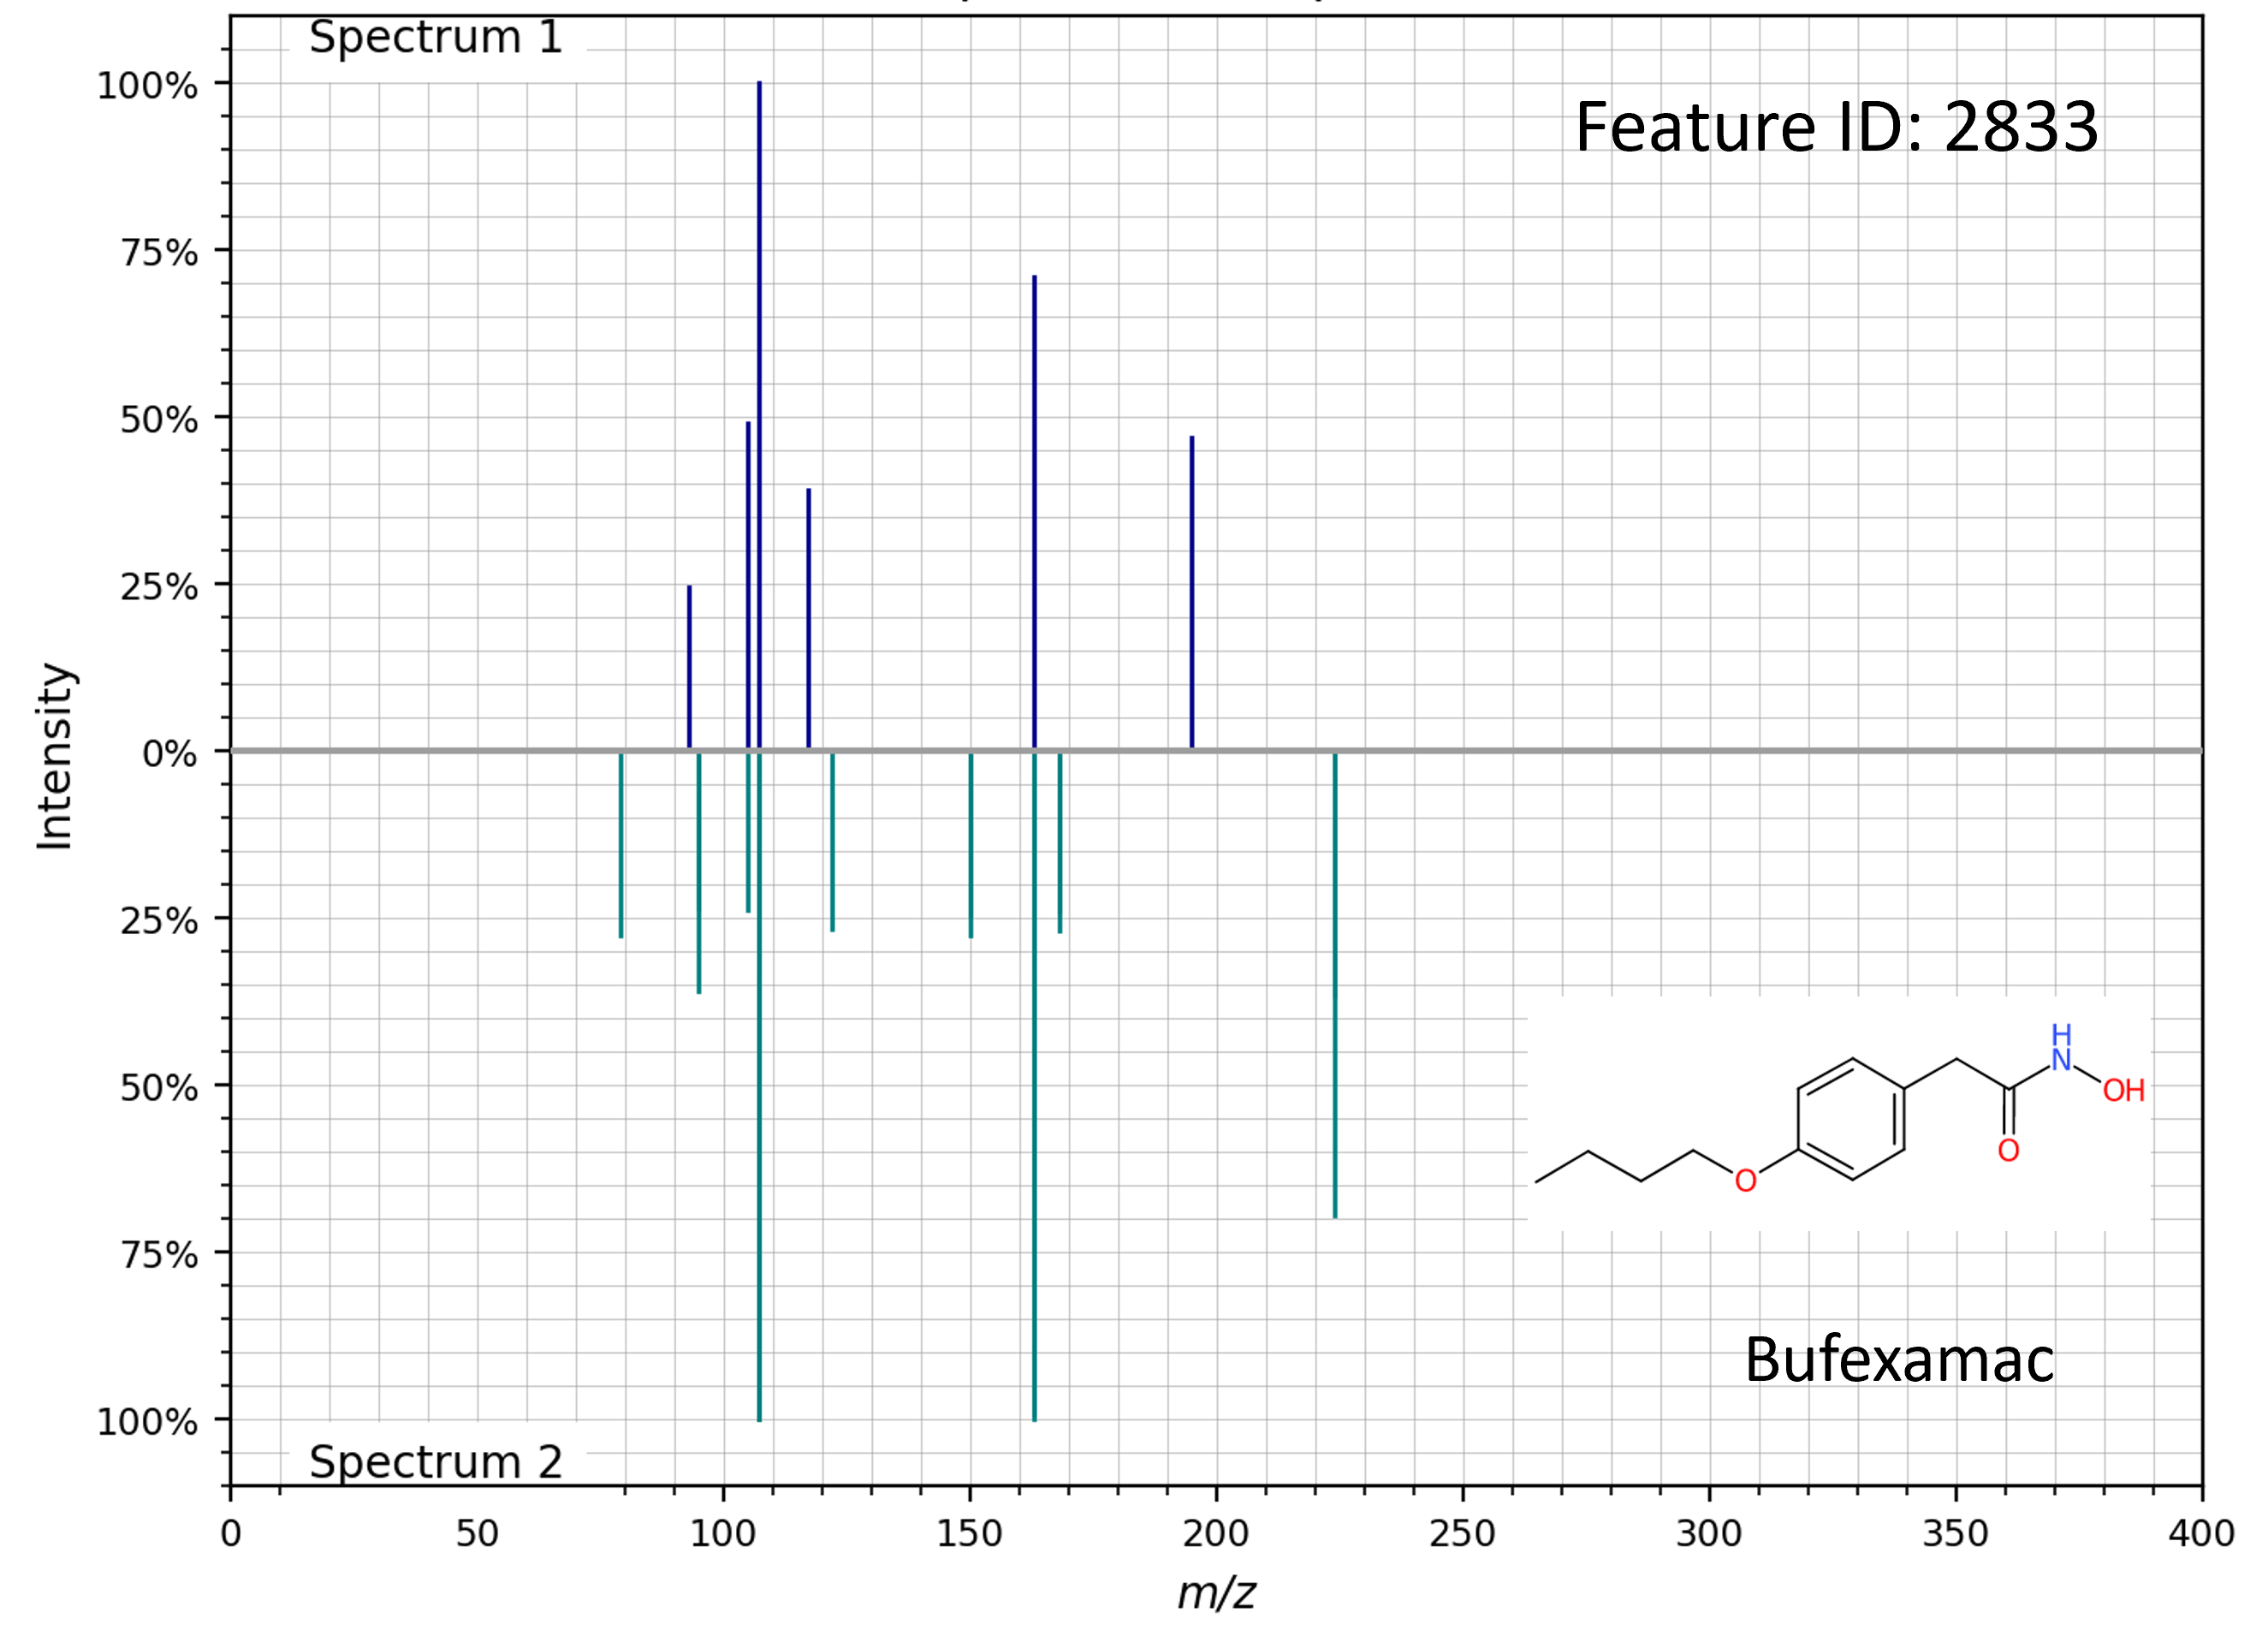
\includegraphics[width=0.8\textwidth]{include/img/appendix/sample/spectra_sample_bufexamac.png}
  \caption{Comparison of a sample feature with a reference spectra (bufexamac: inactive for NR.AR). The figure exemplifies the cases where the number of peaks in the sample feature and the reference node are comparable leading to high cosine scores.}
  \label{fig:sample_spectra_bufexamac}
\end{figure}


\begin{figure}[h]
  \centering
  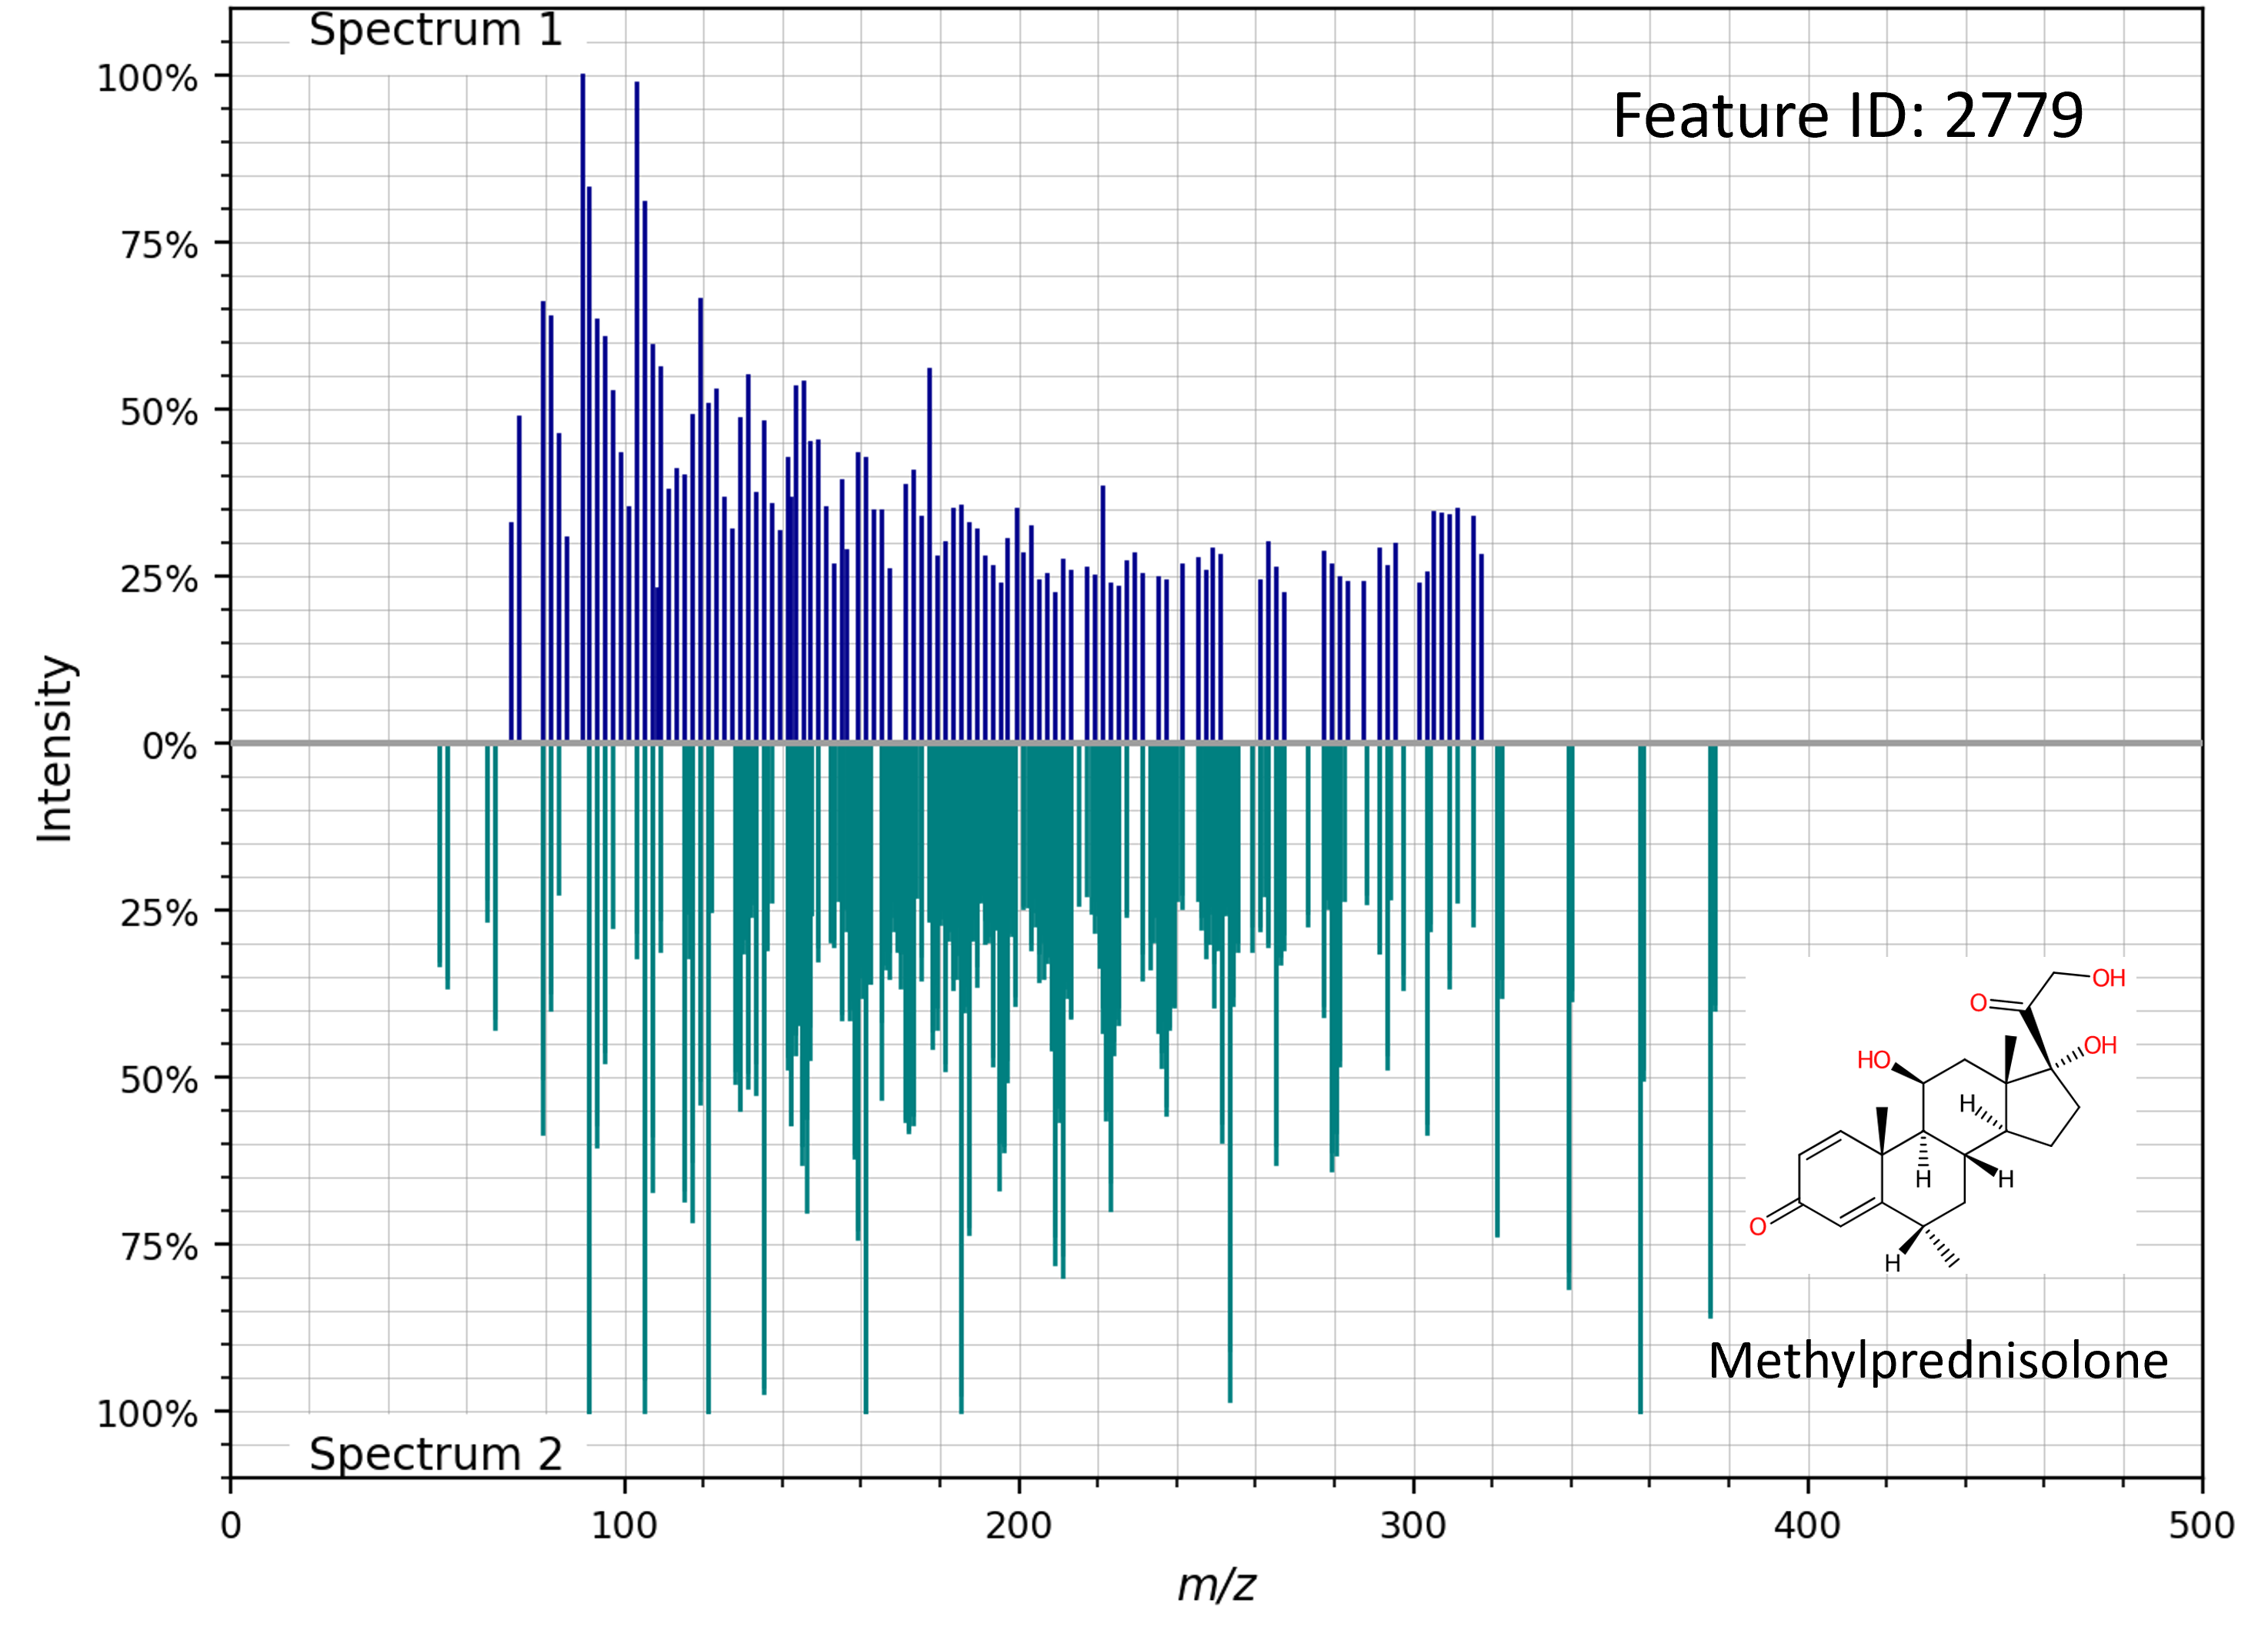
\includegraphics[width=0.8\textwidth]{include/img/appendix/sample/spectra_sample_steroid.png}
  \caption{Comparison of a sample feature with a reference spectra (methylprednisolone: active for NR.AR). This pair exemplifies the cases where the sample features and reference node have a high number of peaks. This could result in a high number of matched peaks but low to medium cosine scores. The number of matched peaks could be then used to associate the detected compounds with the reference network.}
  \label{fig:spectra_sample_steroid}
\end{figure}






